% Basic seminar paper template
% Christian Plessl <christian.plessl@uni-paderborn.de>
%
% based on a template by Holger Karl, (c) 2001

\documentclass[12pt,twoside]{article}
\usepackage{url}


%%%%%%%%%%%%%%%%%%%%%%%%%%%%%%%%%%%%%%%%%%%%%%%%%%%%%%%%%%%%%%%%%%%%%%%%%%%%%%
%%%%%%%%% configure these settings and you are good to go %%%%%%%%%%%%%%%%%%%%
%%%%%%%%%%%%%%%%%%%%%%%%%%%%%%%%%%%%%%%%%%%%%%%%%%%%%%%%%%%%%%%%%%%%%%%%%%%%%%
\newcommand{\participant}{Joe Sample}
\newcommand{\affiliation}{Paderborn University}
\urldef{\emailaddress}\url{joe.sample@uni-paderborn.de}
\newcommand{\topic}{Recent Advances in Custom Computing}


%%%%%%%%%%%%%%%%%%%%%%%%%%%%%%%%%%%%%%%%%%%%%%%%%%%%%%%%%%%%%%%%%%%%%%%%%%%%%%
%%%%%%%%% don't make any other changes in the following   %%%%%%%%%%%%%%%%%%%%
%%%%%%%%% preamble unless you know what you are doing     %%%%%%%%%%%%%%%%%%%%
%%%%%%%%%%%%%%%%%%%%%%%%%%%%%%%%%%%%%%%%%%%%%%%%%%%%%%%%%%%%%%%%%%%%%%%%%%%%%%

\usepackage[english]{babel}
\usepackage[T1]{fontenc}
\usepackage[utf8]{inputenc}
\usepackage{times}

\usepackage{geometry}
\geometry{a4paper,body={15cm,22cm}}

\usepackage{graphicx}
\usepackage{paralist}
\usepackage{fancyhdr}
\pagestyle{fancy}
\fancyhead{}
\fancyhead[LE]{ \slshape \participant}
\fancyhead[LO]{}
\fancyhead[RE]{}
\fancyhead[RO]{ \slshape \topic}
\fancyfoot[C]{}

\begin{document}

\title{\topic}
\author{\Large{\participant}\\ \affiliation \\ {\small \emailaddress}}
\date{}
\maketitle
\thispagestyle{empty}

%%%%%%%%%%%%%%%%%%%%%%%%%%%%%%%%%%%%%%%%%%%%%%%%%%%%%%%%%%%%%%%%%%%%%%%%%%%%%%
%%%%%%%%% here starts the actual text                     %%%%%%%%%%%%%%%%%%%%
%%%%%%%%%%%%%%%%%%%%%%%%%%%%%%%%%%%%%%%%%%%%%%%%%%%%%%%%%%%%%%%%%%%%%%%%%%%%%%

% Abstract gives a brief summary of the main points of a paper:
\begin{abstract}
  The abstract summarizes the contents of the paper in one or two paragraphs.
\end{abstract}

% the actual content, usually separated over a number of sections
% each section is assigned a label, in order to be able to put a
% crossreference to it

\section{Introduction}
\label{sec:introduction}

The introduction describes the problem, why it is important, the main
ideas of the following paper, what are the main contributions of the
paper, etc.

\section{Related Work}
\label{sec:relwork}

The related work section could describe other work that is in some
respects relevant for the understanding of the problem outlined in
Section~\ref{sec:introduction}, that offer competing solutions, etc.

All sources must be properly referenced, ideally by using the BiBTeX
system. References can then be very conveniently made with the
\texttt{\\cite} command. For example, Tobi Oetikers excellent introduction
to \LaTeX can be referenced like this \cite{lshort}.

\section{Model description}
\label{sec:model}

After the two common sections Introduction and Related work, more
sections with the actual content of a paper follow. The style and
structure of such sections varies by a large degree, no general rules
of thumb can be given.

\subsection{How to include figures}

Such a section could, among other things, include a figure. Note that
a figure is a so-called floating object: it is moved around the actual
text in order to best fit on a page. This is in stark contrast to some
GUI-based word processing tools, where the placement of figures is
usually more associated with luck than principle.

As figures float around, expressions like ``the following figure''
must never be used. Instead, figures need a caption, a label, and must
be properly referenced in the main text. An example for this concept
is shown in Figure~\ref{fig:example}.

\begin{figure}
	\centering
	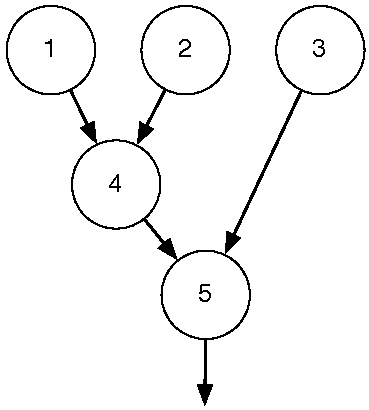
\includegraphics[width=0.3\linewidth]{fig/example}
	\caption{An example figure with a caption.}
	\label{fig:example}
\end{figure}

In general, only vector graphics in PDF format should be included in any
kind of text, as this allows arbitrary scaling, rotation etc.\ without any
loss of quality. Bitmap formats
(JPEG, GIF, \dots) should only be used if no other alternative exists
--- basically the only case where bitmaps can be justified is when
scanned pictures need to be included in a text, however, this should
be avoided as hard as possible as the quality in usually not
satisfactory.

\subsection{How to include tables}

Another frequent element in scientific texts is a table. Like figures, tables are
floating objects that can be moved around in the text by LaTeX to optimize the layout.
For example, see Table~\ref{tab:participants}.

\begin{table}
	\centering
	\begin{tabular}{|c|c|c|}
		\hline
		Name & Matr. No & Email \\
		\hline \hline
		Joe Sample & 654332 & joe.sample\@uni-paderborn.de \\
		Random Guy & 639734 & random.guy\@uni-paderborn.de \\
		John Doe   & 690727 & john.doe\@uni-paderborn.de \\
		\hline
	\end{tabular}
	\caption{Current list of participants in the lecture introduction to computer networks}
	\label{tab:participants}
\end{table}


\subsection{How to create enumerations and itemized lists}

Some procedures become clearer if you put them in an enumerated list, for example, how to eat a cookie:
\begin{enumerate}
	\item buy a cookie,
	\item eat cookie,
	\item remove crumbles.
\end{enumerate}

Similarly, the \texttt{itemize} environment allows for creating non numerated lists.
However, by default, the spacing between the individual items is pretty large. The
\texttt{paralist} package provides alternative, more compact lists and enumerations,
like this:

\begin{compactenum}
	\item buy a cookie,
	\item eat cookie,
	\item remove crumbles.
\end{compactenum}


\section{Further reading for getting started with \LaTeX}
\label{sec:latex}

This document has already introduced the most important constructs of
\LaTeX. What is necessary to produce documents with \LaTeX is a text editor
and a \LaTeX distribution. This is commonly installed on practically all
UNIX-type systems; for Windows, an excellent \LaTeX distribution called
MikTeX is available from \url{www.miktex.org}. Almost all distributions
come with a large patch of examples and introductory material; consult your
local installation for details.

Some people prefer to have an integrated editing environment for \LaTeX which
integrates a text editor with a previewer component. One application that can be
recommended for this purpose is Texmaker \url{http://www.xm1math.net/texmaker/} which
is available for all major operating systems.

For making your next steps with \LaTeX I highly recommend a booklet \cite{lshort} named the
\emph{Not So Short Introduction to \LaTeX2e} which is available online: \url{http://tobi.oetiker.ch/lshort/lshort.pdf}.


\section{Conclusion}
\label{sec:concl}

At the end, there is a final section concluding and summarizing a
paper, putting the entire work into perspective and explaining, on a
larger level, what the consequences of this work are. Also, unexpected
results can be discussed here, etc.


%% the following commands include the biliographic information (in BibTeX format) from the
%% file template.bib
\bibliography{template}
\bibliographystyle{plain}

\end{document}
